\documentclass[twocolumn,superscriptaddress,linenumbers]{revtex4-1} 


\usepackage{hyperref}
\usepackage{verbatim}
\usepackage[font=normalsize]{caption}
\usepackage{mathtools}
\usepackage{relsize}
\usepackage{natbib}

\usepackage{amsmath}
\usepackage{graphicx}
\usepackage[capposition=bottom]{floatrow}
\usepackage{amssymb}
\usepackage{graphicx}
\usepackage{caption}
\usepackage{rotating}
\usepackage{afterpage}
\usepackage{float}
\usepackage{geometry}
\usepackage{titlesec}
\usepackage{epstopdf}

\usepackage{latexsym}
\usepackage{graphicx}
\usepackage{color}
\usepackage{array}
\usepackage{multirow}
\usepackage{wasysym}
\usepackage{verbatim}
\usepackage{subfig}


%switch from two to one column



\addtolength{\oddsidemargin}{-.500in}
\addtolength{\evensidemargin}{-.375in}
\addtolength{\textwidth}{1.00in}
%\addtolength{\voffset}{-70pt}
%\addtolength{\textheight} {120pt}
\newcommand{\isot}[2]{$^{#2}$#1 }
\newcommand{\xeiso}{\isot{Xe}{136}}
\newcommand{\thsrc}{\isot{Th}{228}}
\newcommand{\cosrc}{\isot{Co}{60}}
\newcommand{\krsrc}{\isot{Kr}{83m}}
\newcommand{\cssrc}{\isot{Cs}{137}}
\newcommand{\kevee}{keV$_{ee}$ }
\newcommand{\nonubb}  {$0\nu \beta \beta$}
\newcommand{\gone}{$0.116 \pm 0.003$}
\newcommand{\gtwo}{$11.41 \pm 0.52$}
\newcommand{\fixit}[1]{{\color{red}#1}} 

\renewcommand\thesection{\Roman{section}.}
\renewcommand\thesubsection{\arabic{subsection}.}
\renewcommand\thesubsubsection{\alph{subsubsection}.}
\titleformat{\section}[block]{\bfseries\filcenter}{\thesection}{1em}{}
\titleformat{\subsection}[block]{\bfseries\filcenter}{\thesubsection}{1em}{}
\titleformat{\subsubsection}{\bfseries\filcenter}{\thesubsubsection}{1em}{}

\usepackage{titlesec}

%\titleformat{\section}{\bfseries\filcenter}{\thesubsection}{1em}{}
%\titleformat{\subsection}{\bfseries\filcenter}{\thesubsection}{1em}{}
%\titleformat*{\paragraph}{\large\bfseries}
%\titleformat*{\subparagraph}{\large\bfseries}

\begin{document}

\title{Tritium calibration of the LUX dark matter experiment}

\author{D.S.~Akerib} %% Joined 4/2008
\affiliation{Case Western Reserve University, Dept. of Physics, 10900 Euclid Ave, Cleveland OH 44106, USA}
\affiliation{SLAC National Accelerator Laboratory, 2575 Sand Hill Road, Menlo Park CA 94205-7015, USA}
\affiliation{Kavli Institute for Particle Astrophysics and Cosmology, Stanford University, 452 Lomita Mall, Stanford, CA 94309, USA}

\author{H.M.~Ara\'{u}jo} %% Joined 4/2012, Author on 4/2013
\affiliation{Imperial College London, High Energy Physics, Blackett Laboratory, London SW7 2BZ, UK}

\author{X.~Bai} %% Joined 7/2009
\affiliation{South Dakota School of Mines and Technology, 501 East St Joseph St., Rapid City SD 57701, USA}

\author{A.J.~Bailey} %% Joined 1/2013, Author on 1/2014
\affiliation{Imperial College London, High Energy Physics, Blackett Laboratory, London SW7 2BZ, UK}

\author{J.~Balajthy} %% Joined 7/2012, Author on 7/2013
\affiliation{University of Maryland, Dept. of Physics, College Park MD 20742, USA}

%\author{S.~Bedikian} %% Left 2/2010, Author until 2/2012
%\affiliation{Yale University, Dept. of Physics, 217 Prospect St., New Haven CT 06511, USA}

\author{P.~Beltrame} %% Joined 10/2013, Author on 10/2014.
\affiliation{SUPA, School of Physics and Astronomy, University of Edinburgh, Edinburgh, EH9 3FD, UK}

\author{E.P.~Bernard} %% Joined 1/2010, Author on 1/2011
\affiliation{Yale University, Dept. of Physics, 217 Prospect St., New Haven CT 06511, USA}

\author{A.~Bernstein} %% From the start
\affiliation{Lawrence Livermore National Laboratory, 7000 East Ave., Livermore CA 94551, USA}

\author{T.P.~Biesiadzinski} %% Joined 10/2013, Author on 10/2014
\affiliation{Case Western Reserve University, Dept. of Physics, 10900 Euclid Ave, Cleveland OH 44106, USA}
\affiliation{SLAC National Accelerator Laboratory, 2575 Sand Hill Road, Menlo Park CA 94205-7015, USA}
\affiliation{Kavli Institute for Particle Astrophysics and Cosmology, Stanford University, 452 Lomita Mall, Stanford, CA 94309, USA}

%\author{A.~Bolozdynya} %% From the start, Left Case 7/09, Author until 7/11
%\affiliation{Case Western Reserve University, Dept. of Physics, 10900 Euclid Ave, Cleveland OH 44106, USA}

\author{E.M.~Boulton} %% Joined 3/2013, Author on 3/2014
\affiliation{Yale University, Dept. of Physics, 217 Prospect St., New Haven CT 06511, USA}

\author{A.~Bradley} %% From start, Left 12/2013, Author until 12/2015
\affiliation{Case Western Reserve University, Dept. of Physics, 10900 Euclid Ave, Cleveland OH 44106, USA}

\author{R.~Bramantei} %% Joined 3/2014, Author on 3/2015
\affiliation{Case Western Reserve University, Dept. of Physics, 10900 Euclid Ave, Cleveland OH 44106, USA}
\affiliation{SLAC National Accelerator Laboratory, 2575 Sand Hill Road, Menlo Park CA 94205-7015, USA}
\affiliation{Kavli Institute for Particle Astrophysics and Cosmology, Stanford University, 452 Lomita Mall, Stanford, CA 94309, USA}

%\author{D.~Byram} %% Joined 10/2010, Left 3/2013, Author until 3/2015
%\affiliation{University of South Dakota, Dept. of Physics, 414E Clark St., Vermillion SD 57069, USA}

\author{S.B.~Cahn} %% Joined 2/2009, Left 12/2012, Worked on Kr source in 2015, Author until 12/2017
\affiliation{Yale University, Dept. of Physics, 217 Prospect St., New Haven CT 06511, USA}

\author{M.C.~Carmona-Benitez} %% Joined 10/2009, Moved from Case to UCSB 7/31/2013
\affiliation{University of California Santa Barbara, Dept. of Physics, Santa Barbara, CA, USA}

%\author{D. Carr}{ %% From start, Left on ??
%\affiliation{Lawrence Livermore National Laboratory, 7000 East Ave., Livermore CA 94551, USA}}

\author{C.~Chan} %% Joined 8/2012, Author on 8/2013
\affiliation{Brown University, Dept. of Physics, 182 Hope St., Providence RI 02912, USA}

\author{J.J.~Chapman} %% Joined 6/2007, Author on 6/2008, Left on 1/2014, Author until 1/2016
\affiliation{Brown University, Dept. of Physics, 182 Hope St., Providence RI 02912, USA}

\author{A.A.~Chiller} %% Joined 11/2011, Author on 11/2012
\affiliation{University of South Dakota, Dept. of Physics, 414E Clark St., Vermillion SD 57069, USA}

\author{C.~Chiller} %% Joined 11/2011, Author on 11/2012
\affiliation{University of South Dakota, Dept. of Physics, 414E Clark St., Vermillion SD 57069, USA}

%\author{K.~Clark} %% Joined 6/2008, Left 6/2010, Author until 6/2012
%\affiliation{Case Western Reserve University, Dept. of Physics, 10900 Euclid Ave, Cleveland OH 44106, USA}

%\author{T.~Classen}{ %% Joined 10/2007, Left 11/2009, Author until 11/2011
%  address={University of California Davis, Dept. of Physics, One Shields Ave., Davis CA 95616, USA}}

%\author{T.~Coffey} %% Joined 8/2010, Left 8/2012, Author until 8/2014
%\affiliation{Case Western Reserve University, Dept. of Physics, 10900 Euclid Ave, Cleveland OH 44106, USA}

\author{A.~Currie} %% Joined 4/2012, Author on 4/2013
\affiliation{Imperial College London, High Energy Physics, Blackett Laboratory, London SW7 2BZ, UK}

%\author{A.~Curioni} %% Left 6/2009, Author until 6/2011
%\affiliation{Yale University, Dept. of Physics, 217 Prospect St., New Haven CT 06511, USA}

\author{J.E.~Cutter}  %% Joined 8/2013, Author on 8/2014
\affiliation{University of California Davis, Dept. of Physics, One Shields Ave., Davis CA 95616, USA}

%\author{E.~Dahl}{ %% From start; Left ???
%\affiliation{Case Western Reserve University, Dept. of Physics, 10900 Euclid Ave, Cleveland OH 44106, USA}}

\author{T.J.R.~Davison} %% Joined 2/2014, Author on 2/2015.
\affiliation{SUPA, School of Physics and Astronomy, University of Edinburgh, Edinburgh, EH9 3FD, UK}

%\author{S.~Dazeley} %% From start, Left ?
%\affiliation{Lawrence Livermore National Laboratory, 7000 East Ave., Livermore CA 94551, USA}

\author{L.~de\,Viveiros} %% From the start (at Brown), moved to Coimbra, Left 11/2013, Author until 11/2015. 
\affiliation{LIP-Coimbra, Department of Physics, University of Coimbra, Rua Larga, 3004-516 Coimbra, Portugal}

\author{A.~Dobi} %% Joined 7/2011, Author on 7/2012
\affiliation{Lawrence Berkeley National Laboratory, 1 Cyclotron Rd., Berkeley, CA 94720, USA}

\author{J.E.Y.~Dobson} %% Joined 09/2012, Author on 09/2013, Left 7/2015, Author until 7/2017
\affiliation{Department of Physics and Astronomy, University College London, Gower Street, London WC1E 6BT, UK}

%\author{E.~Dragowsky} %% Joined 01/09, Left 10/11, Author until 10/13
%\affiliation{Case Western Reserve University, Dept. of Physics, 10900 Euclid Ave, Cleveland OH 44106, USA}

\author{E.~Druszkiewicz} %% From the start
\affiliation{University of Rochester, Dept. of Physics and Astronomy, Rochester NY 14627, USA}

\author{B.N.~Edwards} %% Joined 3/2011, Author on 3/2012.
\affiliation{Yale University, Dept. of Physics, 217 Prospect St., New Haven CT 06511, USA}

\author{C.H.~Faham} %% Joined June 2007, Moved from Brown to Berkeley 9/1/2013, Left 6/2015, Author until 6/2017
\affiliation{Lawrence Berkeley National Laboratory, 1 Cyclotron Rd., Berkeley, CA 94720, USA}

\author{S.~Fiorucci} %% From start
\affiliation{Brown University, Dept. of Physics, 182 Hope St., Providence RI 02912, USA}

%\author{C.~Flores} %% Joined 10/2012, Left 10/2012
%\affiliation{University of California Davis, Dept. of Physics, One Shields Ave., Davis CA 95616, USA}

\author{R.J.~Gaitskell} %% From start
\affiliation{Brown University, Dept. of Physics, 182 Hope St., Providence RI 02912, USA}

\author{V.M.~Gehman} %% Joined 5/2012, Author on 5/2013, Left 6/2015, Author until 6/2017
\affiliation{Lawrence Berkeley National Laboratory, 1 Cyclotron Rd., Berkeley, CA 94720, USA}

\author{C.~Ghag} %% Joined 6/2012, Author on 6/2013
\affiliation{Department of Physics and Astronomy, University College London, Gower Street, London WC1E 6BT, UK}

\author{K.R.~Gibson} %% Joined 10/2009, Left 9/2014, Author until 9/2016
\affiliation{Case Western Reserve University, Dept. of Physics, 10900 Euclid Ave, Cleveland OH 44106, USA}

\author{M.G.D.~Gilchriese} %% Joined 10/2010, Author on 10/2011
\affiliation{Lawrence Berkeley National Laboratory, 1 Cyclotron Rd., Berkeley, CA 94720, USA}

\author{C.R.~Hall} %% Joined 3/2008, Author on 3/2009
\affiliation{University of Maryland, Dept. of Physics, College Park MD 20742, USA}

\author{M.~Hanhardt} %% Joined 7/2009, Left 8/2011, Rejoined 7/2013, Author on 7/2014
\affiliation{South Dakota School of Mines and Technology, 501 East St Joseph St., Rapid City SD 57701, USA}
\affiliation{South Dakota Science and Technology Authority, Sanford Underground Research Facility, Lead, SD 57754, USA}

\author{S.J.~Haselschwardt}  %% Joined 6/2013, Author on 6/2014
\affiliation{University of California Santa Barbara, Dept. of Physics, Santa Barbara, CA, USA}

\author{S.A.~Hertel} %% Joined 9/2012, Author on 9/2013
\affiliation{University of California Berkeley, Department of Physics, Berkeley, CA 94720, USA}
\affiliation{Yale University, Dept. of Physics, 217 Prospect St., New Haven CT 06511, USA}

\author{D.P.~Hogan} %% Joined 2/2014, Author on 2/2015
\affiliation{University of California Berkeley, Department of Physics, Berkeley, CA 94720, USA}

%\author{B.~Holbrook}{ %% Engineer, Joined 12/2007
%  address={University of California Davis, Dept. of Physics, One Shields Ave., Davis CA 95616, USA}}

\author{M.~Horn} %% Joined 4/2012, Author on 4/2013.
\affiliation{University of California Berkeley, Department of Physics, Berkeley, CA 94720, USA}
\affiliation{Yale University, Dept. of Physics, 217 Prospect St., New Haven CT 06511, USA}

\author{D.Q.~Huang} %% Joined 7/2012, Author on 7/2013
\affiliation{Brown University, Dept. of Physics, 182 Hope St., Providence RI 02912, USA}

\author{C.M.~Ignarra} %% Joined 10/2014, Author on 10/2015
\affiliation{SLAC National Accelerator Laboratory, 2575 Sand Hill Road, Menlo Park CA 94205-7015, USA}
\affiliation{Kavli Institute for Particle Astrophysics and Cosmology, Stanford University, 452 Lomita Mall, Stanford, CA 94309, USA}

\author{M.~Ihm} %% Joined 10/2009, Author on 10/2010
\affiliation{University of California Berkeley, Department of Physics, Berkeley, CA 94720, USA}

%\author{T. Ivancic}{ %% Joined 1/2012, Left 6/2012, Never an author.
%  address={Case Western Reserve University, Dept. of Physics, 10900 Euclid Ave, Cleveland OH 44106, USA}}

\author{R.G.~Jacobsen} %% Joined 12/2009, Author on 12/2010
\affiliation{University of California Berkeley, Department of Physics, Berkeley, CA 94720, USA}

\author{W.~Ji} %% Joined 3/2014, Author on 3/2015
\affiliation{Case Western Reserve University, Dept. of Physics, 10900 Euclid Ave, Cleveland OH 44106, USA}
\affiliation{SLAC National Accelerator Laboratory, 2575 Sand Hill Road, Menlo Park CA 94205-7015, USA}
\affiliation{Kavli Institute for Particle Astrophysics and Cosmology, Stanford University, 452 Lomita Mall, Stanford, CA 94309, USA}

%\author{K.~Kamdin %% Joined 3/2015, Author on 3/2016
%\affiliation{University of California Berkeley, Department of Physics, Berkeley, CA 94720, USA}

%\author{L.~Kastens} %% Joined 6/2007, Left 7/2011, Author until 7/2013
%\affiliation{Yale University, Dept. of Physics, 217 Prospect St., New Haven CT 06511, USA}

\author{K.~Kazkaz} %% From start
\affiliation{Lawrence Livermore National Laboratory, 7000 East Ave., Livermore CA 94551, USA}

\author{D.~Khaitan} %% Joined 6/2014, Author on 6/2015
\affiliation{University of Rochester, Dept. of Physics and Astronomy, Rochester NY 14627, USA}

\author{R.~Knoche} %% Joined 7/2011, Author on 7/2012
\affiliation{University of Maryland, Dept. of Physics, College Park MD 20742, USA}

%\author{S.~Kyre} %% Engineer, Joined 6/2010
%\affiliation{University of California Santa Barbara, Dept. of Physics, Santa Barbara, CA, USA}

%\author{R.~Lander} %% Joined 3/2008, Decided not to be a LUX author.
%\affiliation{University of California Davis, Dept. of Physics, One Shields Ave., Davis CA 95616, USA}

\author{N.A.~Larsen} %% Joined 6/2010, Author on 6/2011
\affiliation{Yale University, Dept. of Physics, 217 Prospect St., New Haven CT 06511, USA}

\author{C.~Lee} %% Joined 8/2009
\affiliation{Case Western Reserve University, Dept. of Physics, 10900 Euclid Ave, Cleveland OH 44106, USA}
\affiliation{SLAC National Accelerator Laboratory, 2575 Sand Hill Road, Menlo Park CA 94205-7015, USA}
\affiliation{Kavli Institute for Particle Astrophysics and Cosmology, Stanford University, 452 Lomita Mall, Stanford, CA 94309, USA}

\author{B.G.~Lenardo} %% Joined 7/2013, Author on 7/2014
\affiliation{University of California Davis, Dept. of Physics, One Shields Ave., Davis CA 95616, USA}
\affiliation{Lawrence Livermore National Laboratory, 7000 East Ave., Livermore CA 94551, USA}

%\author{D.S.~Leonard} %% Joined 11/2008, Left 2/2010, Author until 2/2012.
%\affiliation{University of Maryland, Dept. of Physics, College Park MD 20742, USA}

\author{K.T.~Lesko} %% Joined 3/2007, Left ?, Rejoined 4/2013, Author on 4/2014
\affiliation{Lawrence Berkeley National Laboratory, 1 Cyclotron Rd., Berkeley CA 94720, USA}

\author{A.~Lindote} %% Joined 12/2010, Author on 12/2011.
\affiliation{LIP-Coimbra, Department of Physics, University of Coimbra, Rua Larga, 3004-516 Coimbra, Portugal}

\author{M.I.~Lopes} %% Joined 12/2010, Author on 12/2011.
\affiliation{LIP-Coimbra, Department of Physics, University of Coimbra, Rua Larga, 3004-516 Coimbra, Portugal}

%\author{R. Lorek}{ %% Joined 6/2012, Focussed on R&D for LZ, Will not be an author.
%  address={Case Western Reserve University, Dept. of Physics, 10900 Euclid Ave, Cleveland OH 44106, USA}}

%\author{A.~Lyashenko} %% Joined 7/2009, Left 8/2011, Author until 8/2013
%\affiliation{Yale University, Dept. of Physics, 217 Prospect St., New Haven CT 06511, USA}

\author{D.C.~Malling} %% Joined 8/2007, Author on 8/2008, Left on 12/2013, Author until 12/2015 
\affiliation{Brown University, Dept. of Physics, 182 Hope St., Providence RI 02912, USA}

\author{A.G.~Manalaysay}{ %% Joined 10/2013, Author on 10/2014
\affiliation{University of California Davis, Dept. of Physics, One Shields Ave., Davis CA 95616, USA}}

\author{R.L.~Mannino} %% Joined 6/2009, Author on 6/2010
\affiliation{Texas A \& M University, Dept. of Physics, College Station TX 77843, USA}

\author{M.F.~Marzioni} %% Joined 9/2014, Author on 9/2015
\affiliation{SUPA, School of Physics and Astronomy, University of Edinburgh, Edinburgh, EH9 3FD, UK}

\author{D.N.~McKinsey} %% Joined 6/2007, Author on 6/2008
\affiliation{University of California Berkeley, Department of Physics, Berkeley, CA 94720, USA}
\affiliation{Yale University, Dept. of Physics, 217 Prospect St., New Haven CT 06511, USA}

\author{D.-M.~Mei} %% Joined 7/2008
\affiliation{University of South Dakota, Dept. of Physics, 414E Clark St., Vermillion SD 57069, USA}

\author{J.~Mock} %% Joined 8/2007
\affiliation{University at Albany, State University of New York, Dept. of Physics, 1400 Washington Ave., Albany, NY 12222, USA}

\author{M.~Moongweluwan} %% Joined 6/2011, Author on 6/2012.
\affiliation{University of Rochester, Dept. of Physics and Astronomy, Rochester NY 14627, USA}

\author{J.A.~Morad} %% Joined 7/2012, Author on 7/2013
\affiliation{University of California Davis, Dept. of Physics, One Shields Ave., Davis CA 95616, USA}

%\author{M.~Morii} %% Joined June 09, Left May 2011, Author until May 2013
%\affiliation{Harvard University, Dept. of Physics, 17 Oxford St., Cambridge MA 02138, USA}

\author{A.St.J.~Murphy} %% Joined 06/2012, Author on 06/2013.
\affiliation{SUPA, School of Physics and Astronomy, University of Edinburgh, Edinburgh, EH9 3FD, UK}

\author{C.~Nehrkorn} %% Joined 5/2012, Author on 5/2013
\affiliation{University of California Santa Barbara, Dept. of Physics, Santa Barbara, CA, USA}

\author{H.N.~Nelson} %% Joined 11/2008
\affiliation{University of California Santa Barbara, Dept. of Physics, Santa Barbara, CA, USA}

\author{F.~Neves} %% Joined 12/2010, Author on 12/2011.
\affiliation{LIP-Coimbra, Department of Physics, University of Coimbra, Rua Larga, 3004-516 Coimbra, Portugal}

%\author{J.A.~Nikkel} %% Joined 4/2008, Left 12/2011, Author until 12/2013
%\affiliation{Yale University, Dept. of Physics, 217 Prospect St., New Haven CT 06511, USA}

\author{K.~O'Sullivan} %% Joined 9/2012, Author on 9/2013
\affiliation{University of California Berkeley, Department of Physics, Berkeley, CA 94720, USA}
\affiliation{Lawrence Berkeley National Laboratory, 1 Cyclotron Rd., Berkeley CA 94720, USA}
\affiliation{Yale University, Dept. of Physics, 217 Prospect St., New Haven CT 06511, USA}

\author{K.C.~Oliver-Mallory} %% Joined 5/2014, Author on 5/2015
\affiliation{University of California Berkeley, Department of Physics, Berkeley, CA 94720, USA}

\author{R.A.~Ott} %% Joined 3/2012, Author on 3/2013, Left on 3/2014, Author until 3/2016
\affiliation{University of California Davis, Dept. of Physics, One Shields Ave., Davis CA 95616, USA}

\author{K.J.~Palladino} %% Joined 10/2013, Author on 10/2014
\affiliation{SLAC National Accelerator Laboratory, 2575 Sand Hill Road, Menlo Park CA 94205-7015, USA}
\affiliation{Kavli Institute for Particle Astrophysics and Cosmology, Stanford University, 452 Lomita Mall, Stanford, CA 94309, USA}

\author{M.~Pangilinan} %% Joined 2/2010, Left  4/2014, Author until 4/2016
\affiliation{Brown University, Dept. of Physics, 182 Hope St., Providence RI 02912, USA}

%\author{P.D.~Parker} %% Joined 9/2010, Active on 12/2011, Left on 6/2013, Author until 6/2015
%\affiliation{Yale University, Dept. of Physics, 217 Prospect St., New Haven CT 06511, USA}

\author{E.K.~Pease} %% Joined 12/2011, Author on 12/2012.
\affiliation{Yale University, Dept. of Physics, 217 Prospect St., New Haven CT 06511, USA}

%\author{K.~Pech} %% Joined 6/2011, Author on 6/2012, Left 9/2013, Author until 9/2015
%\affiliation{Case Western Reserve University, Dept. of Physics, 10900 Euclid Ave, Cleveland OH 44106, USA}

\author{P.~Phelps} %% Joined 6/2008, Left 7/2014, Author until 7/2016
\affiliation{Case Western Reserve University, Dept. of Physics, 10900 Euclid Ave, Cleveland OH 44106, USA}

%\author{J.~Pinto~da~Cunha}{ %% Joined 12/2010, will not be an author until further notice.
%\affiliation{LIP-Coimbra, Department of Physics, University of Coimbra, Rua Larga, 3004-516 Coimbra, Portugal}}

\author{L.~Reichhart} %% Joined 6/2012, Author on 6/2013, Left on 5/2015, Author until 5/2017
\affiliation{Department of Physics and Astronomy, University College London, Gower Street, London WC1E 6BT, UK}

\author{C.~Rhyne} %% Joined 6/2014, Author on 6/2015
\affiliation{Brown University, Dept. of Physics, 182 Hope St., Providence RI 02912, USA}

\author{S.~Shaw} %% Joined 2/2014, Author on 2/2015
\affiliation{Department of Physics and Astronomy, University College London, Gower Street, London WC1E 6BT, UK}

\author{T.A.~Shutt} %% From start
\affiliation{Case Western Reserve University, Dept. of Physics, 10900 Euclid Ave, Cleveland OH 44106, USA}
\affiliation{SLAC National Accelerator Laboratory, 2575 Sand Hill Road, Menlo Park CA 94205-7015, USA}
\affiliation{Kavli Institute for Particle Astrophysics and Cosmology, Stanford University, 452 Lomita Mall, Stanford, CA 94309, USA}

\author{C.~Silva} %% Joined 12/2010, Author on 12/2011.
\affiliation{LIP-Coimbra, Department of Physics, University of Coimbra, Rua Larga, 3004-516 Coimbra, Portugal}

%\author{W.~Skulski} %% From start, Author on trigger-related publications.
%\affiliation{University of Rochester, Dept. of Physics and Astronomy, Rochester NY 14627, USA}

\author{V.N.~Solovov} %% Joined 12/2010, Author on 12/2011.
\affiliation{LIP-Coimbra, Department of Physics, University of Coimbra, Rua Larga, 3004-516 Coimbra, Portugal}

\author{P.~Sorensen} %% From start
\affiliation{Lawrence Berkeley National Laboratory, 1 Cyclotron Rd., Berkeley, CA 94720, USA}

%\author{J. Spaans} %% Joined 2/2009, Left 5/2010, Author until 5/2012
%\affiliation{University of South Dakota, Dept. of Physics, 414E Clark St., Vermillion SD 57069, USA}}

\author{S.~Stephenson}  %% Joined 8/2014, Author on 8/2015
\affiliation{University of California Davis, Dept. of Physics, One Shields Ave., Davis CA 95616, USA}

%\author{T. Stiegler} %% Joined 10/2007, Left on 12/2011, Not authorship
%\affiliation{Texas A \& M University, Dept. of Physics, College Station TX 77843, USA}

\author{T.J.~Sumner} %% Joined 4/2012, Author on 4/2013
\affiliation{Imperial College London, High Energy Physics, Blackett Laboratory, London SW7 2BZ, UK}

%\author{R.~Svoboda} %% From start, Decided not to be a LUX author.
%\affiliation{University of California Davis, Dept. of Physics, One Shields Ave., Davis CA 95616, USA}

%\author{M.~Sweany} %% From start, Left 6/11, Author until 6/13
%\affiliation{University of California Davis, Dept. of Physics, One Shields Ave., Davis CA 95616, USA}

\author{M.~Szydagis} %% Joined 5/2010, Author on 5/2011
\affiliation{University at Albany, State University of New York, Dept. of Physics, 1400 Washington Ave., Albany, NY 12222, USA}

\author{D.J.~Taylor} %% Joined 3/2010, Author on 3/2011
\affiliation{South Dakota Science and Technology Authority, Sanford Underground Research Facility, Lead, SD 57754, USA}

\author{W.~Taylor} %% Joined 6/14, Author on 6/15
\affiliation{Brown University, Dept. of Physics, 182 Hope St., Providence RI 02912, USA}

\author{B.P.~Tennyson} %% Joined 6/2012, Author on 6/2013
\affiliation{Yale University, Dept. of Physics, 217 Prospect St., New Haven CT 06511, USA}

\author{P.A.~Terman} %% Joined 1/2014, Author on 1/2015
\affiliation{Texas A \& M University, Dept. of Physics, College Station TX 77843, USA}

\author{D.R.~Tiedt}  %% Joined 10/2012, Author on 10/2013
\affiliation{South Dakota School of Mines and Technology, 501 East St Joseph St., Rapid City SD 57701, USA}

%\author{J.~Thomson}{ %% Engineer, Joined 5/2008
%  address={University of California Davis, Dept. of Physics, One Shields Ave., Davis CA 95616, USA}}

\author{W.H.~To} %% Joined 10/2013, Author on 10/2014
\affiliation{Case Western Reserve University, Dept. of Physics, 10900 Euclid Ave, Cleveland OH 44106, USA}
\affiliation{SLAC National Accelerator Laboratory, 2575 Sand Hill Road, Menlo Park CA 94205-7015, USA}
\affiliation{Kavli Institute for Particle Astrophysics and Cosmology, Stanford University, 452 Lomita Mall, Stanford, CA 94309, USA}

\author{M.~Tripathi} %% From start
\affiliation{University of California Davis, Dept. of Physics, One Shields Ave., Davis CA 95616, USA}

\author{L.~Tvrznikova} %% Joined 10/2013, Author on 10/2014
\affiliation{Yale University, Dept. of Physics, 217 Prospect St., New Haven CT 06511, USA}

\author{S.~Uvarov} %% Joined 7/2009, Author on 7/2010
\affiliation{University of California Davis, Dept. of Physics, One Shields Ave., Davis CA 95616, USA}

\author{J.R.~Verbus} %% Joined 7/09
\affiliation{Brown University, Dept. of Physics, 182 Hope St., Providence RI 02912, USA}

%\author{N.~Walsh} %% Joined 2/2008, Left 10/2012, Author until 10/2014
%\affiliation{University of California Davis, Dept. of Physics, One Shields Ave., Davis CA 95616, USA}

\author{R.C.~Webb} %% Joined 4/2008
\affiliation{Texas A \& M University, Dept. of Physics, College Station TX 77843, USA}

\author{J.T.~White} %% From start
\affiliation{Texas A \& M University, Dept. of Physics, College Station TX 77843, USA}

%\author{D.~White} %% Engineer, Joined 6/2010
%\affiliation{University of California Santa Barbara, Dept. of Physics, Santa Barbara, CA, USA}

\author{T.J.~Whitis} %% Joined 9/2013, Author on 9/2014
\affiliation{Case Western Reserve University, Dept. of Physics, 10900 Euclid Ave, Cleveland OH 44106, USA}
\affiliation{SLAC National Accelerator Laboratory, 2575 Sand Hill Road, Menlo Park CA 94205-7015, USA}
\affiliation{Kavli Institute for Particle Astrophysics and Cosmology, Stanford University, 452 Lomita Mall, Stanford, CA 94309, USA}

\author{M.S.~Witherell} %% Joined 3/2012, Author on 3/2013
\affiliation{University of California Santa Barbara, Dept. of Physics, Santa Barbara, CA, USA}

%\author{M.~Wlasenko} %% Joined 10/2009, Left 5/2011, Author until 5/2013
%\affiliation{Harvard University, Dept. of Physics, 17 Oxford St., Cambridge MA 02138, USA}

\author{F.L.H.~Wolfs} %% From start
\affiliation{University of Rochester, Dept. of Physics and Astronomy, Rochester NY 14627, USA}

%\author{M.~Woods} %% Joined 10/2008, Left 9/2013, Author until 9/2015
%\affiliation{University of California Davis, Dept. of Physics, One Shields Ave., Davis CA 95616, USA}

%\author{J.~Xu} %% Joined 9/2015, Author on 9/2016
%\affiliation{Lawrence Livermore National Laboratory, 7000 East Ave., Livermore CA 94551, USA}

%\author{K.~Yazdani} %% Joined 12/2014, Author on 12/2015
%\affiliation{Imperial College London, High Energy Physics, Blackett Laboratory, London SW7 2BZ, UK}

\author{M.~Yen} %% Joined 5/2014, Author on 5/2015
\affiliation{University of California Berkeley, Department of Physics, Berkeley, CA 94720, USA}

\author{S.K.~Young} %% Joined 8/2014, Author on 8/2015
\affiliation{University at Albany, State University of New York, Dept. of Physics, 1400 Washington Ave., Albany, NY 12222, USA}

\author{C.~Zhang} %% Joined 2/2009
\affiliation{University of South Dakota, Dept. of Physics, 414E Clark St., Vermillion SD 57069, USA}


 \begin{abstract}

We present measurements of the electron-recoil (ER) response of the LUX dark matter detector using an internal tritium calibration source. The large-statistics tritium dataset provides ideal single-beta events with high purity and good spatial uniformity. We report on the charge and light yields of liquid xenon at 180 V/cm and 105 V/cm with high accuracy down to 1.3~keV energies, investigate fluctuations in the ER band, measure the energy threshold of the detector, and validate the combined energy model. These results provide input to the LUX Run3 WIMP search \cite{lux-reanalysis}.

\end{abstract}



%\twocolumn[\maketitle]
		\maketitle


\section{Introduction}

The Large Underground Xenon experiment (LUX) is a WIMP search located at the 4850' level of the Sanford Underground Research Facility (SURF) in Lead, South Dakota~\cite{lux-nim}. LUX detects particle interactions in liquid xenon (LXe) via scintillation (S1) and ionization charge (S2) signals. The LXe is instrumented as a dual-phase time projection chamber (TPC), providing an energy measurement, position information in three dimensions, and single-scatter event identification. Electron-recoil (ER) and nuclear-recoil (NR) events are distinguished by the ratio of the charge and light signals (S2/S1). Results from the first LUX science run (Run 3) were first reported in Ref.~\cite{lux-prl}. An improved analysis of the Run 3 data is reported in Ref.~\cite{lux-reanalysis}.

The LUX is monitored and calibrated primarily with electron sources that can be dissolved in the LXe. Two such sources,  \krsrc~\cite{Kastens:2009rt, Baudis} and tritium ($^{3}$H), have been deployed in LUX, both providing a large sample of spatially uniform events. In this article we report results from the calibration of LUX with tritium, a single-beta emitter with a Q value of 18.6~keV electron-equivalent\footnote{ER events and NR events generally have different energy scales in LXe. In this article we interpret all events using the ER energy scale.}~\cite{Tritium_Q}. 

The tritium beta spectrum is well known both theoretically and experimentally. It has a broad peak at 2.5~keV and a mean energy of 5.6~keV~\cite{Tritium_Mean,Tritium_Eq,Drexlin:2013lha}. 64.2\% of the decays occur between 1 and 8~keV, the energy range of interest for WIMP searches. These characteristics make it an ideal source for studying the ER response of LUX.  $\rm ^{83m}$Kr, which is a source of 9.4~keV and 32.1~keV internal conversion electrons, is well suited for routine monitoring and for correcting the spatial and temporal variations of the S1 and S2 signals, but is less useful for studies of the S2/S1 ER discrimination variable because both conversion electrons are above the dark matter energy range, and because the S2 signals from the two electrons generally overlap in the detector due to the short half-life of the intermediate state (154~ns). External gamma sources, such as \cssrc,  are also used on occasion by LUX, but they are unable to produce a useful rate of fiducial single-scatter calibration events in LUX in the WIMP energy range of interest due to self-shielding. We note that the most important background in LUX is due to Compton scatters, and such events are expected to have similar properties to beta decays in the tritium energy range. Neutron sources and a neutron generator are also employed by LUX to study the response to NR events~\cite{DD-paper}.

We use tritiated methane (CH$_3$T) as the host molecule to deliver tritium activity into LUX. Compared to molecular tritium (T$_2$), CH$_3$T has several advantages. It does not adsorb onto surfaces like the T$_2$ molecule, and it does not interfere with charge transport in LXe. Also, because of its 12.3 year half-life, tritium must be removed from the detector by purification, and methane is amenable to chemical removal with standard noble gas purifiers~\cite{Dobi_CH4}. Note, however, that diffusion of tritium activity into plastic detector components during the calibration is an important concern, since that activity may later re-contaminate the LXe during the WIMP search runs.  In this respect, CH$_3$T is preferable over T$_2$ due to its larger molecular size and lower diffusion constant and solubility~\cite{miyake:1983}. We investigated the CH$_3$T contamination risk empirically with a series of bench-top tests prior to the first injection into LUX. These tests, which are described in Appendix \ref{sec:appendix1}, demonstrated that the injection and removal could be done without undue risk to the experiment. 

An initial tritium dataset of $\sim$7,000 fiducial events was obtained by LUX in August of 2013, and the results were reported in Ref~\cite{lux-prl}. Subsequently, in December 2013, we injected additional activity with a higher rate and obtained a fiducial tritium dataset of 170,000 events. This dataset is used to characterize the LUX ER band in Ref.~\cite{lux-reanalysis}. Except where otherwise noted, in this article we report results from the larger December 2013 dataset.

\section{Injection and removal of CH$_3$T}

Two CH$_3$T sources with total activities of 3 Bq and 200 Bq were prepared for use in LUX. Each source is contained in a 2.25 liter stainless steel bottle and is mixed with 2 atmospheres of LUX-quality purified xenon. The xenon acts as a carrier gas to extract the source from the bottle. The CH$_3$T was synthesized for LUX by Moravek Biochemical~\cite{moravek} and delivered at a specific activity of 0.1 milliCurie per millimol.

The injection system is shown in Fig.~\ref{fig:plumbing}. A fraction of the source bottle activity may be extracted by allowing the carrier gas to expand into one or more expansion volumes consisting of various sections of evacuated tubing. The amount of extracted activity is controlled by selecting an expansion volume of appropriate size. A methane purifier (SAES model MC1-905F\cite{seas}) located between the source bottle and the expansion volume ensures that only CH$_3$T, CH$_4$, and noble gases are allowed to enter the system. The extracted activity is then injected into the TPC by diverting a small portion of the LUX xenon gas flow through the expansion volumes. 

\begin{figure}[h!]
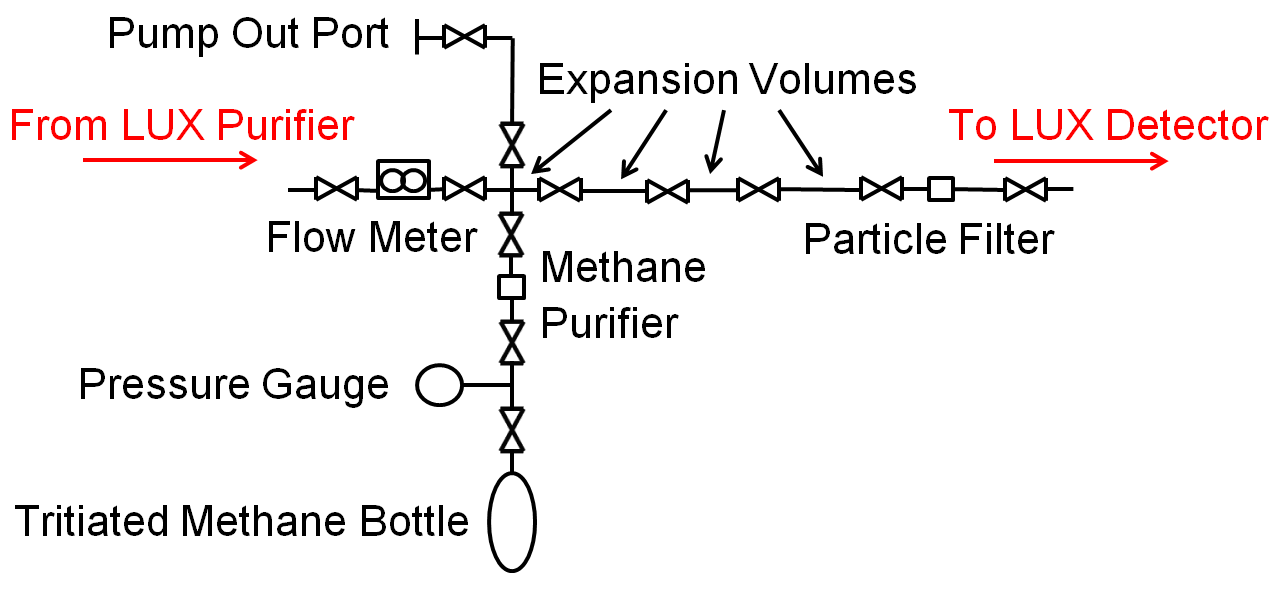
\includegraphics[width=80mm]{fig/TritiumPlumbing.png}
\caption{Plumbing diagram of the CH$_3$T injection system for LUX. CH$_3$T is injected downstream of the xenon gas purifier so that it passes through the detector prior to being removed.  Red arrows indicate the direction of flow.}
\label{fig:plumbing}
\end{figure}

The CH$_3$T appears in the TPC within minutes of the injection, and is removed via the normal action of the LUX xenon purification system, which operates without interruption during the entire procedure. Its centerpiece is a hot zirconium getter (SAES model PS4-MT15-R1\cite{seas}) that acts upon gaseous xenon and continuously removes all non-noble species including methane. The xenon gas flow is driven by a diaphragm pump at a rate of $\sim$27 standard liters per minute. 

Prior to the first injection of CH$_3$T activity, we first confirmed that the LUX getter unit was capable of efficient methane removal by injecting  $\sim$1 ppm (part-per-million g/g) of natural methane (CH$_4$) into LUX. As shown in Fig.~\ref{fig:ch4_removal}, the CH$_4$ concentration in the gas, monitored with a mass spectrometer, was observed  to decrease exponentially with a time constant of 5.9 $\pm 0.07$ hours. The one-pass efficiency of the getter for CH$_4$ removal was measured to be 97\% under the LUX flow and temperature conditions by sampling the gas before and after the getter. 

On August 8, 2013, an initial injection of 20 mBq of CH$_3$T was performed, followed five days later by an injection of 800 mBq. The count rate of fiducial single-scatter events with S1 $<$ 150 photons detected (phd) (roughly the endpoint of the tritium beta spectrum) is shown in Fig.~\ref{fig:ch3t_removal}. The CH$_3$T activity is clearly observed, with the count rate reaching its maximal value in one hour. For both injections the activity was removed with a six-hour exponential time constant similar to that observed in the CH$_4$ injection. It is worth noting that the observed purification time constant is considerably shorter than the xenon mass turn-over time of LUX (about 40 hours for 370 kg of xenon).  The origin of the short purification time remains under investigation. The location of the CH$_3$T events from the first injection after all corrections is shown in Fig.~\ref{fig:event_location}. As expected, the events are uniform within the detector volume.� An empirical model that describes the removal of CH$_3$T from LUX is presented in Appendix~\ref{sec:appendix2}.

\begin{figure}[h!]
<<<<<<< HEAD
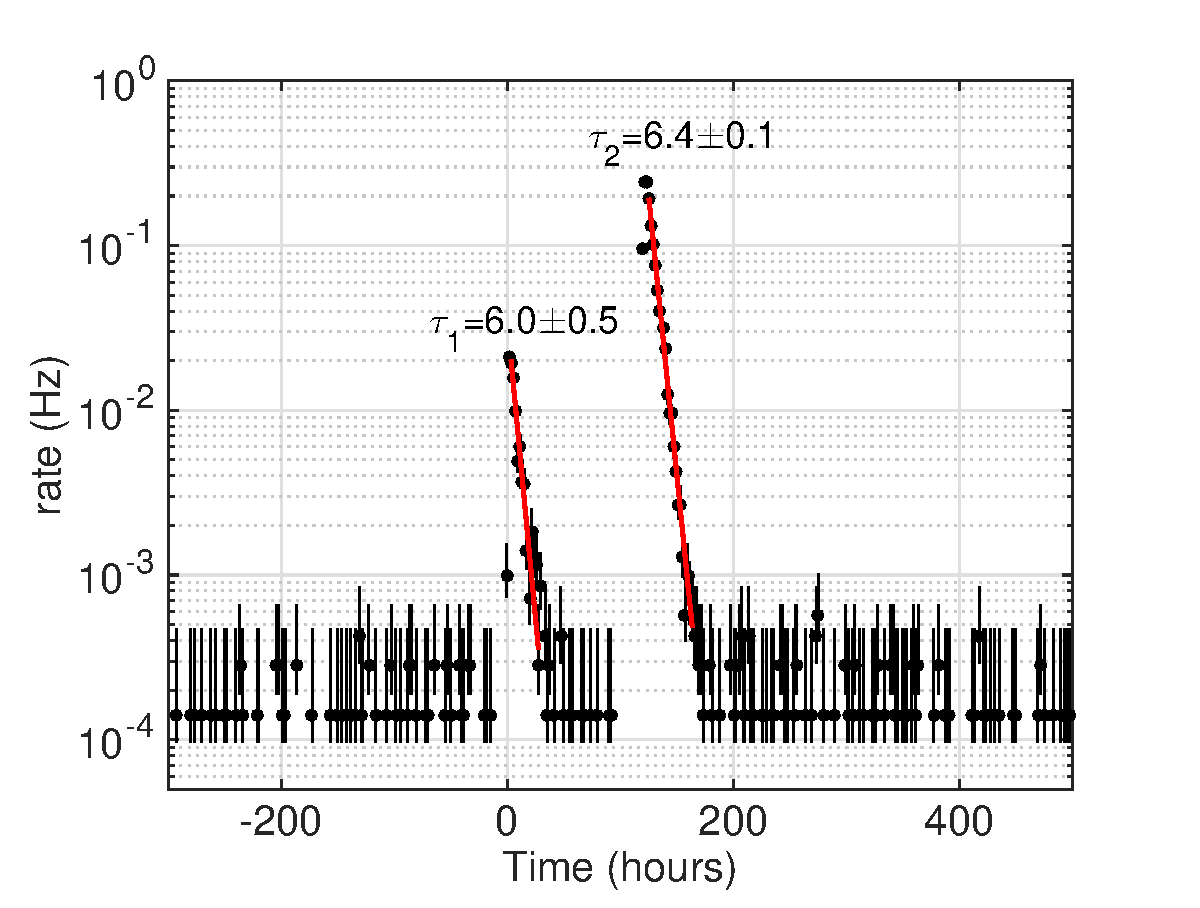
\includegraphics[width=90mm]{fig/CH3T_Rate.eps}
\caption{Rate of single scatter events with S1 below 150 phd in the fiducial volume during the August 2013 CH$_3$T injections.  The magenta and red curves are exponential fits to the activity vs time.}
=======
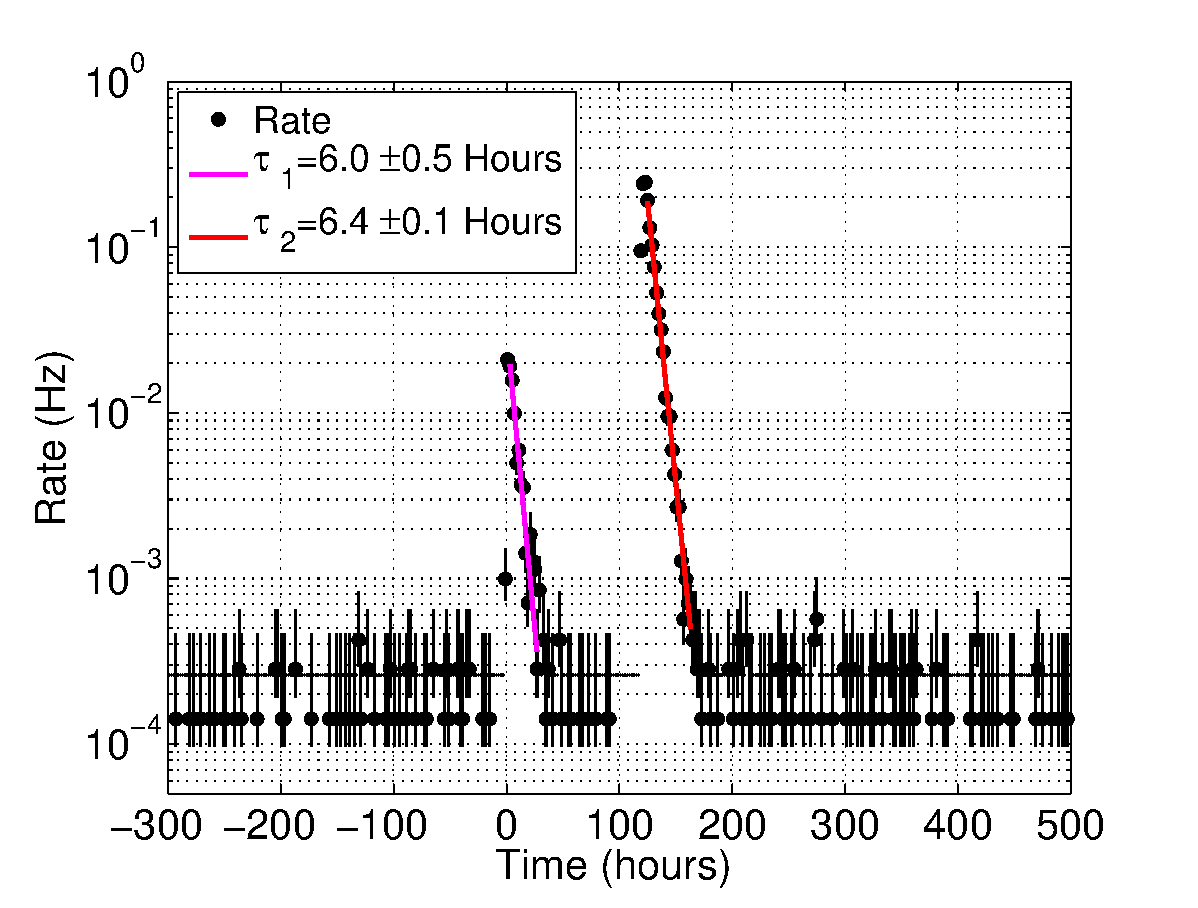
\includegraphics[width=80mm]{fig/CH3T_Rate_fid_150_Run03_Tritium_Rate.eps}
\caption{Rate of single scatter events with S1 below 150 phd in the fiducial volume during the August 2013 CH$_3$T injections.  The magenta and red curves are exponential fits to the activity vs. time.}
>>>>>>> origin/master
\label{fig:ch3t_removal}
\end{figure}


 
\begin{figure}[h!]
<<<<<<< HEAD
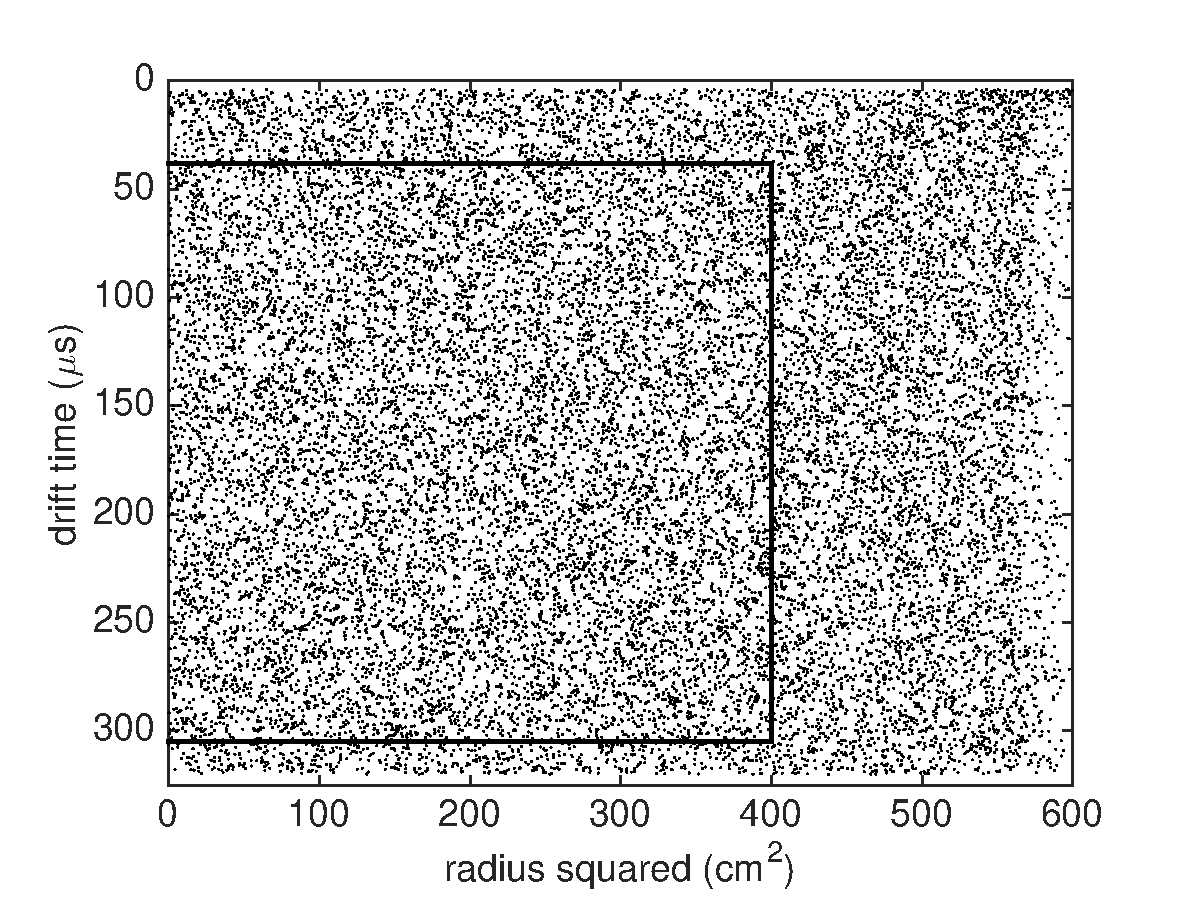
\includegraphics[width=90mm]{fig/rz_scatter.eps}
\caption{The location of events in drift time vs. detector radius squared for the August 2013 CH$_3$T injection. The drift time is a proxy for the $z$ coordinate of the event. The solid black line represents the fiducial volume used in \cite{lux-reanalysis}.}
=======
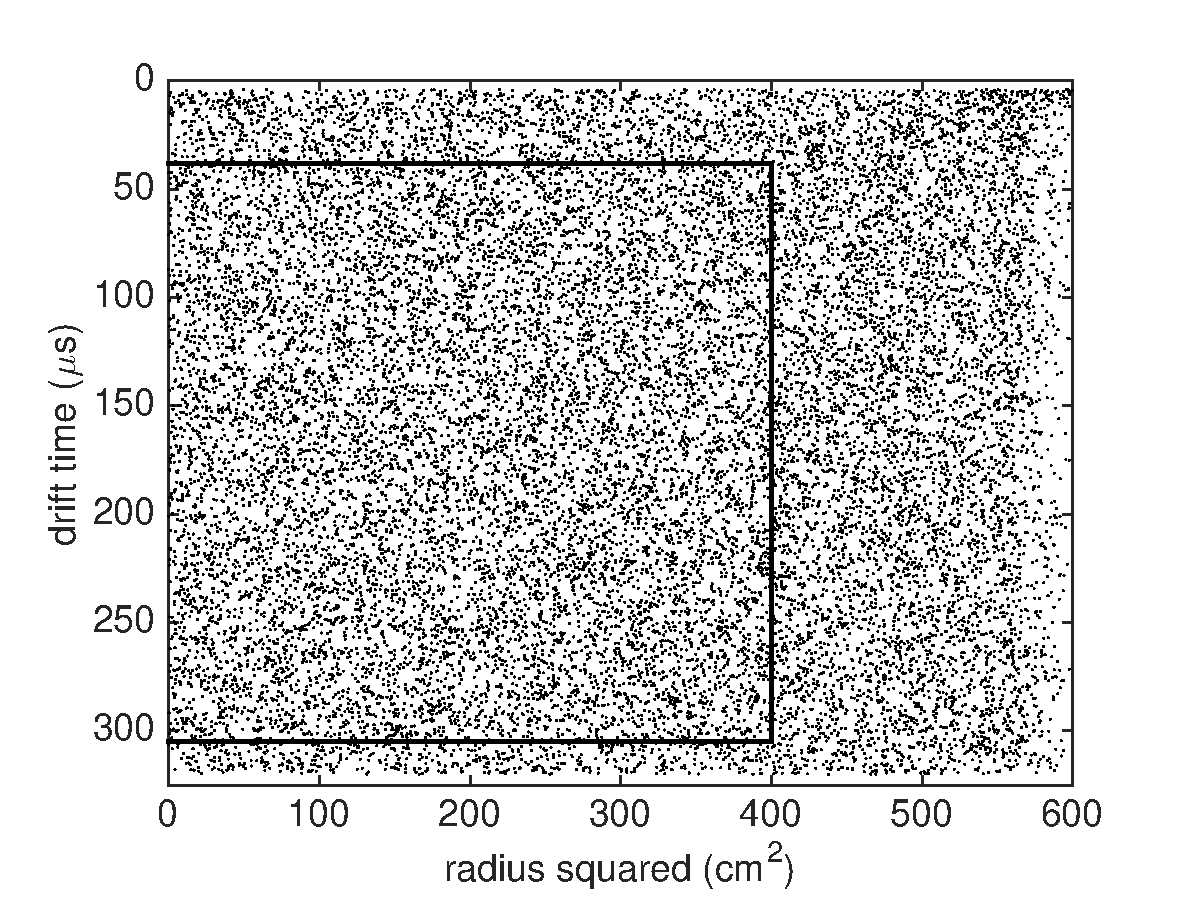
\includegraphics[width=80mm]{fig/rz_scatter.eps}
\caption{The location of events in drift time vs. detector radius squared for the August 2013 CH$_3$T injection. The drift time is a proxy for the $z$ coordinate of the event. The solid black line represents the fiducial volume used in~\cite{lux-reanalysis}.}
>>>>>>> origin/master
\label{fig:event_location}
\end{figure}







\input{results}

\section{Summary}

We have characterized the electron recoil band and threshold of the LUX dark matter experiment with a tritium calibration source. The large dataset, high event purity, and simple topology provide a powerful tool to study the detector and to investigate the fundamental properties of LXe as a particle detection medium. The results presented here are used in an improved analysis of the Run 3 WIMP search data in Ref. \cite{lux-reanalysis}.

\appendix

\section{Studies of the removal of CH$_3$T from LXe }
\label{sec:appendix1}

\newcommand*{\Scale}[2][4]{\scalebox{#1}{$#2$}}%

Prior to the first injection of CH$_3$T into LUX, we considered three risks that such a calibration may pose to the dark matter search: 1) that the xenon purification system may be ineffective for CH$_3$T removal; 2) that the interior surfaces of the stainless steel (SS)  gas handling system may become permanently contaminated with CH$_3$T; and 3) that the plastic detector components may outgas unacceptable quantities of CH$_3$T after initial exposure.

To address the first concern we studied the removal of natural methane (CH$_4$) from Xe gas with a heated Zr getter and a mass spectrometer. The purification efficiency was found to be satisfactory\cite{Dobi_CH4}. Furthermore, a test of the completed LUX purification system, including the actual getter unit, was performed several weeks before the first CH$_3$T injection into LUX. In this test $\sim$0.1 grams of CH$_4$ was injected into LUX, and mass spectrometry measurements of the CH$_4$ concentration in the LUX Xe gas were performed over the next several days. The CH$_4$ concentration was observed to decrease exponentially with a time constant of 5.90 $\pm 0.07$ hours as shown in Fig. \ref{fig:ch4_removal}, confirming the effectiveness of the purification system for methane removal.

The behavior of CH$_3$T in SS plumbing was studied in a bench-test with a custom-built Xe gas proportional tube operated at room temperature. Substantial quantities of CH$_3$T activity were injected, counted, and removed from the proportional tube. Initial tests found a small amount of residual activity after purification, however this was resolved by passing the CH$_3$T through a methane purifier (SAES model MC1-905F). No subsequent contamination was observed.

\begin{figure}[h!]\centering
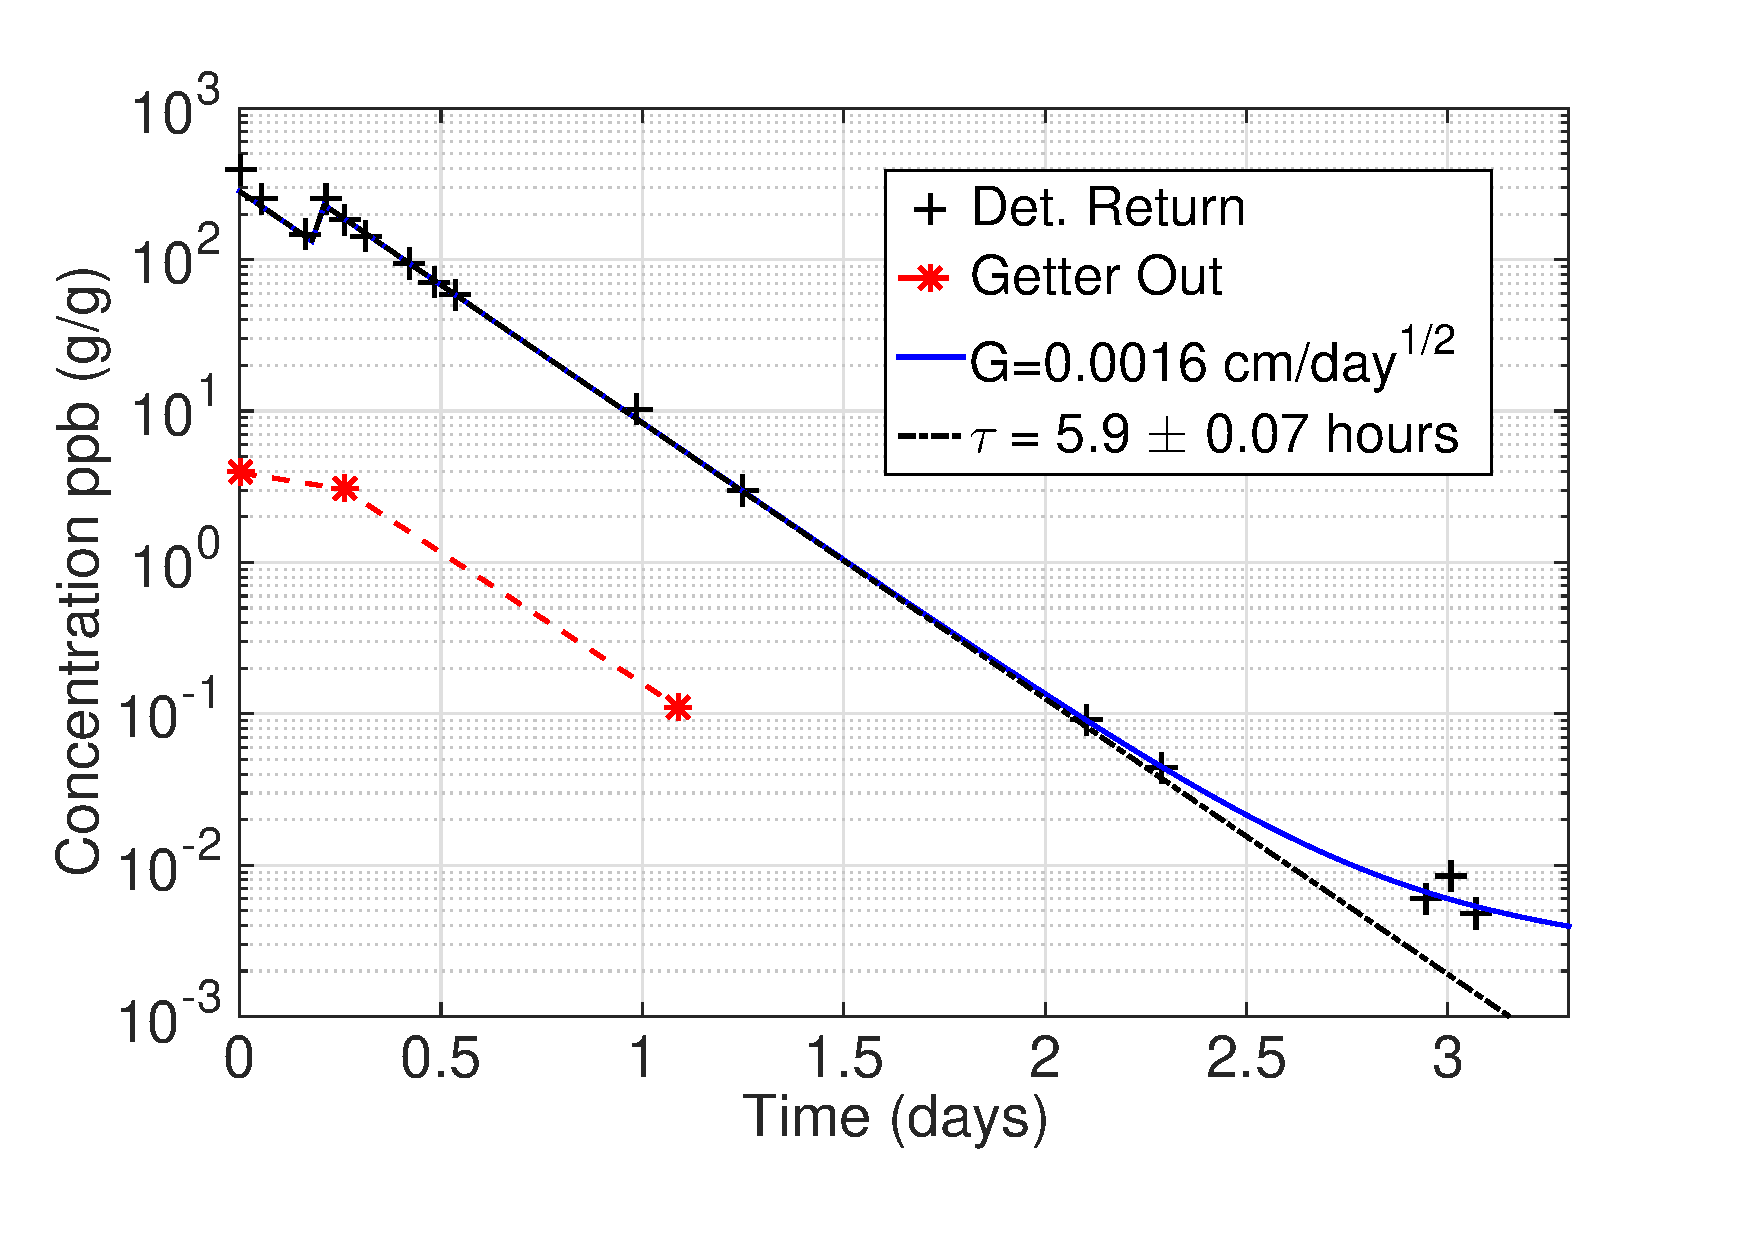
\includegraphics[width=80mm]{fig/July_CH4_wOG.eps}
\caption{Injection and removal of CH$_4$ in LUX prior to the first CH$_3$T injection. CH$_4$ is observed with a gas sampling mass spectrometry system. The black dashed lines shows an exponential fit to the CH$_4$ concentration at the detector return line with a time constant of 5.90 $\pm 0.07$ hours.  The red points indicate measurements at the getter outlet. We find a 97\% one-pass removal efficiency at a flow rate of 27 SLPM. The blue curve shows the upper limit on the effect of outgassing from the plastics. The three data points near t = 3 days are consistent with the limit of detection for methane ($\sim \rm 5\times10^{-3}$ ppb (g/g)) .}
\label{fig:ch4_removal}
\end{figure}

We also performed tests of CH$_3$T injection and removal from LXe with a small detector. One such experiment is shown in Fig. \ref{fig:Density}, where 68,000 Hz of CH$_3$T was injected, counted, and subsequently removed from LXe. Samples of LUX polyethylene and teflon were immersed in the LXe in this experiment, and their outgassing is evident in Fig. \ref{fig:Density}. These data placed constraints on the risk of CH$_3$T outgassing in LUX. In total over one million Hz of CH$_3$T activity was injected and successfully removed in these experiments.

\begin{figure}[h!]\centering
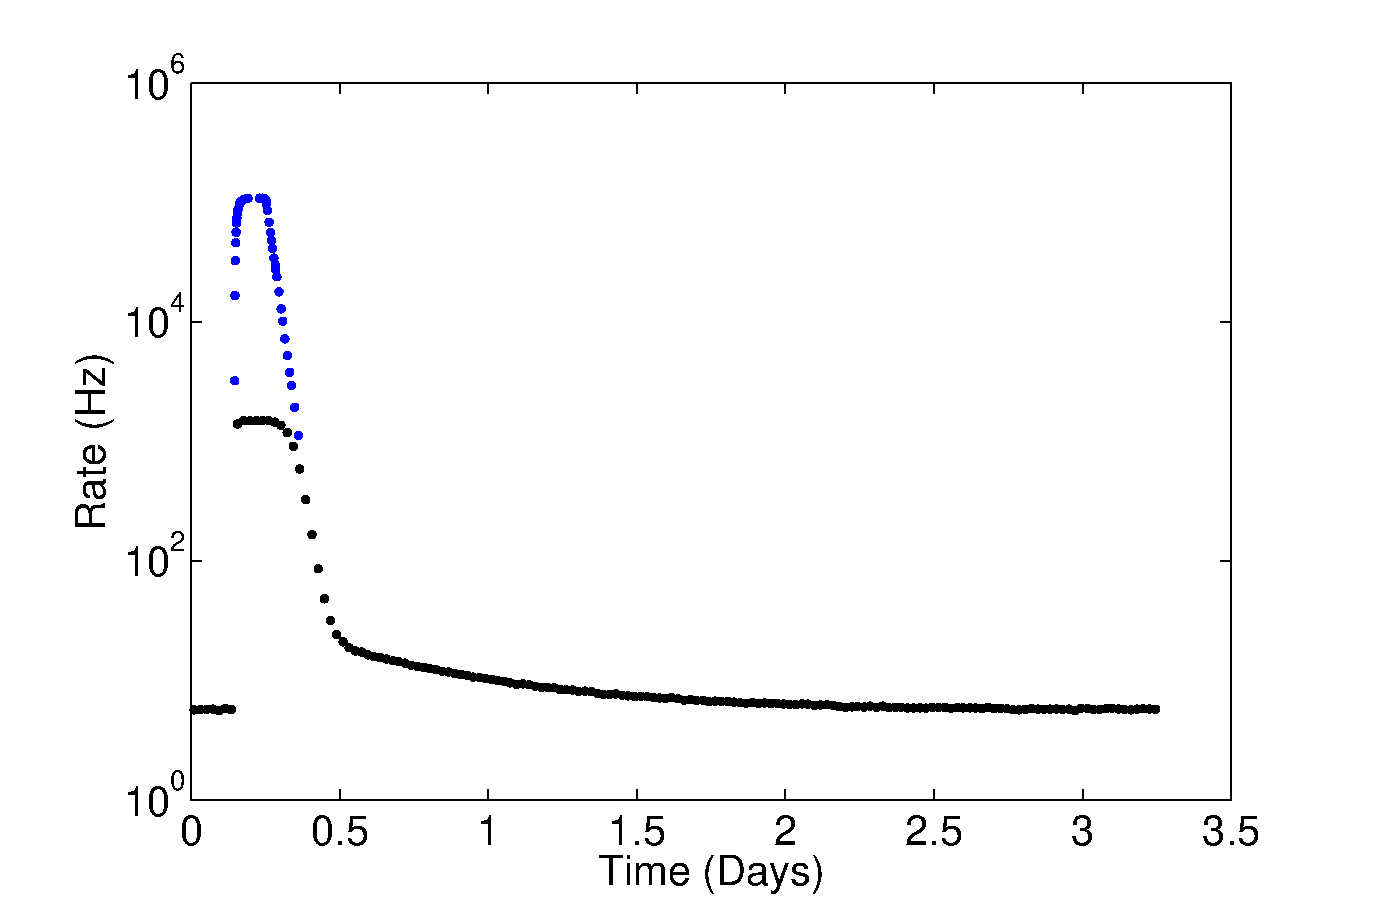
\includegraphics[width=80mm]{fig/TimeHisto_Analog2.eps}
\caption{The event rate versus time following a large CH$_3$T injection into a bench-top liquid xenon detector. Black points: the event rate measured with a dead-time limited digital DAQ system. Blue: true event rate measured with a fast analog scalar. In this experiment a maximum activity of 68,000 Hz was detected immediately after the injection, compared to a background count rate of 5 Hz. Initially the purifier is not included in the recirculation circuit, leading to a constant count rate. The count rate falls rapidly when the purifier is activated. At 0.5 days an elbow in the count rate is observed, indicating that outgassing of CH$_3$T from the detector plastics has become a limiting factor in the purification rate. }
\label{fig:Density}
\end{figure}


\section{Model of CH$_3$T removal}
\label{sec:appendix2}

We use a simple purification model to predict the CH$_3$T activity in LUX after an injection. The model is 

\begin{equation}
\frac{dC}{dt} = \frac{A}{V}J_{out} -\frac{C}{\tau},
\end{equation}

\noindent where  $C$ is the CH$_3$T concentration in the LXe,  $J_{out}$ is the flux of CH$_3$T out of the plastic components due to outgassing,  $A$ is the surface area of the plastic TPC cylinder, $V$ is the total volume of xenon in the active region, and $\tau$ is the characteristic removal time of CH$_3$T due to purification (5.9 hours). The model assumes perfect mixing of the fluid in the TPC. The initial concentration is the injection activity divided by the volume of the active region. We solve the model numerically with the Euler method while simultaneously solving the diffusion equation to determine $J_{out}$. The results predict the number of calibration events that may be collected and provide an estimate of when the CH$_3$T  decay rate will be small enough to allow the WIMP search to resume.

We approximate the diffusion into and out of the plastics as one-dimensional, since most plastics in LUX can be approximated as a thin cylindrical shell with no dependence on the azimuthal or $z$ coordinates.  Fick's laws in one dimension are

\begin{align}
J=-D\frac{d \phi(r,t)}{d r}  \\
\frac{d \phi}{d t} = D \frac{d^2 \phi(r,t)}{d r^2} 
\end{align}

\noindent 
where $J$ is the flux, $\phi(r,t)$ is the CH$_3$T  concentration in the plastic at depth $r$ and time $t$, and $D$ is the diffusion constant in the plastic. The concentration at the LXe-plastic boundary is fixed at $KC$, where K is the unitless solubility of CH$_3$T in the plastics. These equations are solved numerically and simultaneously with the purification model. 

$D$ and $K$ are not independently known for CH$_3$T in teflon or polyethylene at LXe temperature. However, only the combined quantity $G \equiv K \sqrt{ D/ \pi }$ is relevant as long as the diffusing substance does not reach the center of the plastic component (a good assumption for diffusion of CH$_3$T at LXe temperature). Under this condition, there exists an analytic solution to Fick's first law, which we evaluate at the LXe boundary:

%\begin{equation}
%\Scale[0.75]{\phi (x,t) = KC - \int \limits_0^t erf(\frac{x}{\sqrt{4D(t - \tau)}})K\frac{d}{d\tau}C(\tau)d\tau - KC(0)erf(\frac{x}{\sqrt{4Dt}}),}
%\end{equation}

\begin{equation}
J_{out}(t)= - G\left( \int \limits_0^t \frac{\frac{d}{dt'}C(t')}{\sqrt{t-t'}} dt' + \frac{C(0)}{\sqrt{t}}\right),
\end{equation}

\noindent
where the sign is reversed because the flux of material is outward. This result can be derived by applying Duhamel's principle along the infinite half-line, and it shows that the outgassing flux is linear in $G$. We set an upper limit of $G<0.0016 \frac{cm}{\sqrt{day}}$ for LUX based upon the data in Fig. \ref{fig:ch4_removal}. In that data the effect of $G$ would appear as an elbow in the CH$_4$ concentration versus time, as indicated by the blue line. The three data points near t = 3 days constrain the maximum value of $G$. We interpret this result as an upper limit because those data points are consistent with CH$_4$ backgrounds in the mass spectrometry system.

\begin{figure}[h!]
\centering
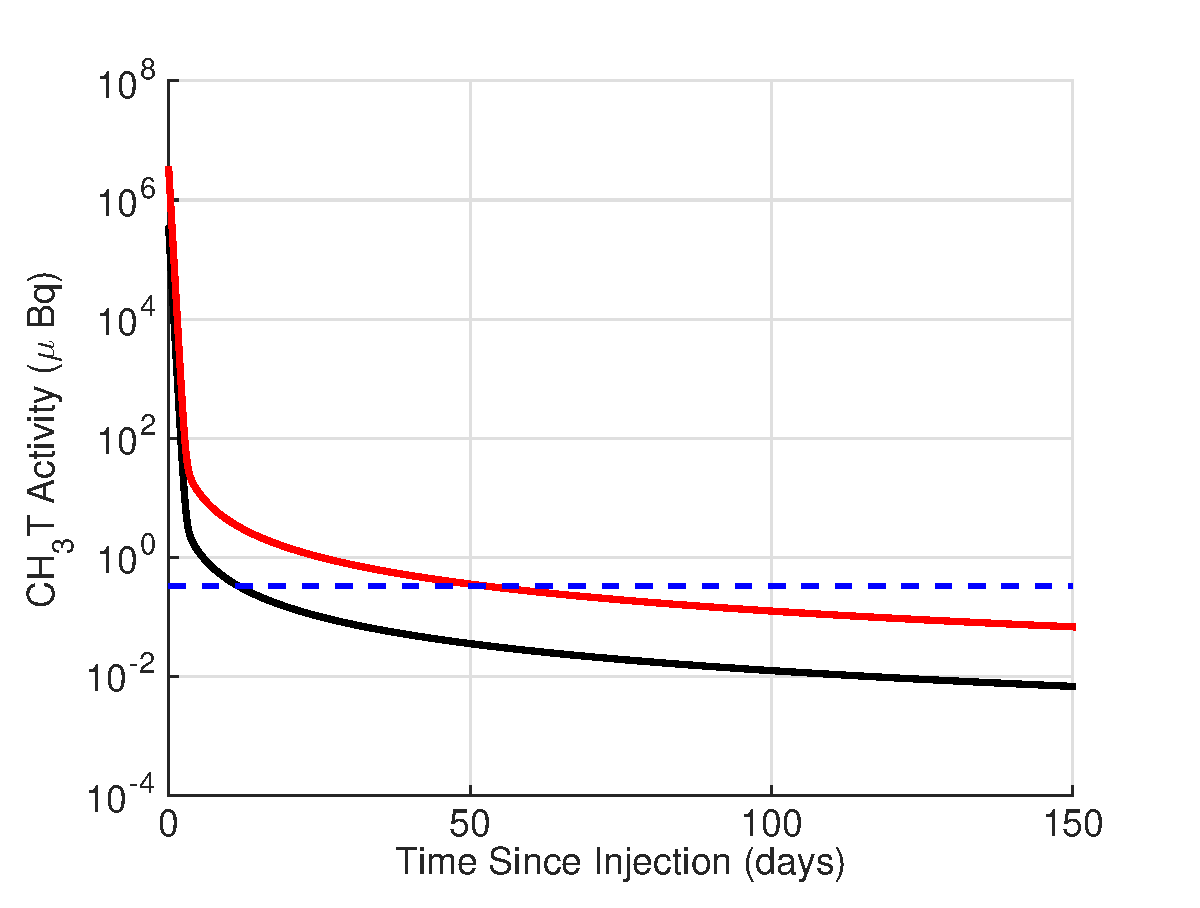
\includegraphics[width=0.95\textwidth]{fig/LUX_og_lim.eps}
\caption{Results of the purification model from 1 Bq (black curve) and 10 Bq (red curve) injections of CH$_3$T into LUX. The dashed blue line is the tritium activity goal of 0.33 $\mu$ Bq. The sharp initial fall is due to the 5.9 hour purification time constant of LUX, while the slow long-term removal is dominated by outgassing. The outgassing simulated here assumes  $G=0.0016$ cm/day$^{1/2}$).}
\label{fig:tau_var}
\end{figure}

Fig. \ref{fig:tau_var} shows the results of the purification model for a 1 Bq and 10 Bq injection into LUX assuming $G$ = 0.0016 cm/day$^{1/2}$  . We take 0.33 $\mu$Bq of residual CH$_3$T activity as an approximate goal for resuming WIMP search running, and we find that for injections on the order of 1 Bq we reach 0.33 $\mu$Bq eight days later, while 10 Bq injections may take as long as 35 days.  Ultimately the final decision regarding low background data quality is made during the data analysis phase, with guidance provided by the purification model described here.

%\begin{acknowledgments}

%\end{acknowledgments}

%double blank page so that the table doesn't spill into the bibliography
\newpage
\thispagestyle{empty}
\mbox{}
\newpage
\thispagestyle{empty}
\mbox{}

\bibliographystyle{thesisbibstyle}
\bibliography{Tritium}

\end{document}